\chapter{Fluids}

a fluid, such as a liquid or a gas, is a substance that has no fixed shape

unlike a solid, a fluid can flow and yield easily under external force

in this chapter, we will study several aspects of a fluid

\subsection{pressure in a fluid}

\begin{marginfigure}
	\vspace*{-8pt}
	\centering
	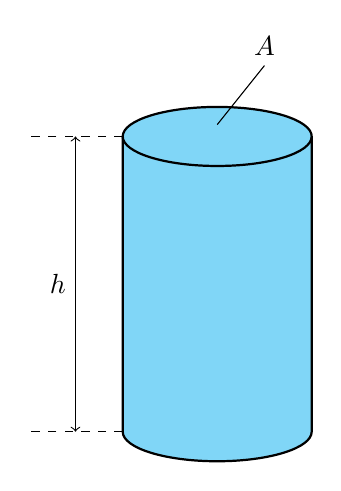
\begin{tikzpicture}[yscale=0.75,xscale=0.6]
	\draw[thick,fill=cyan!50] (-2,2.5) arc(180:0:2 and 0.5) -- (2,-2.5) arc(0:-180:2 and 0.5) -- cycle;
	\draw[thick] (2,2.5) arc(0:-180:2 and 0.5);
	\draw (0,2.7) --++ (1,1) node[above]{$A$};
	\draw[<->] (-3,2.5) -- (-3,-2.5) node[left,midway]{$h$};
	\draw[dashed] (-2,2.5) --++ (-2,0);
	\draw[dashed] (-2,-2.5) --++ (-2,0);
	\end{tikzpicture}
	\vspace*{-16pt}
\end{marginfigure}


at a depth of $h$ below surface of a fluid, self-weight of the fluid could produce a pressure


{
	\centering
	
	$ p = \frac{F}{A} = \frac{mg}{A} = \frac{\rho V g}{A} \RA \boxed{p = \rho g h} $
	
}




\cmt pressure in a liquid depends on depth

for different positions in a liquid, as long as they are at same depth, pressure is the same

i.e., pressure does not depend on volume or shape of container

\cmt atmospheric pressure also accounts for total pressure in a liquid

atmosphere presses on surface of a liquid, so total pressure at depth $h$ is: $P=\rho g h + P_\text{atm}$

nevertheless, change in pressure still satisfies: $\Delta p = \rho g \Delta h$

\example{The atmospheric pressure is about $1.0 \times 10^5 \text{ Pa}$. Given that the density of sea water is $1020 \text{ kg m}^{-3}$, what is the total pressure 50 m below the surface of the sea?}

\solc\begin{equation*}
	P = P_\text{atm} + \rho g h = 1.0 \times 10^5 + 1020 \times 9.81 \times 50 \RA P \approx 6.0 \times 10^5 \text{ Pa} 
\end{equation*}

\example{A vertical column of liquid of height 10 m contains both oil and water. The pressure due to the liquids at the bottom of the column is 89 kPa. Given that the density of water is $1000 \text{ kg m}^{-3}$ and the density of the oil is $840 \text{ kg m}^{-3}$. What is the depth of the oil?}

\solc\begin{equation*}
	P = P_\text{oil} + P_\text{water} = \rho_\text{o} g h_\text{o} + \rho_\text{w} g h_\text{w}
\end{equation*}
\begin{equation*}
840 \times 9.81 \times x + 1000 \times 9.81 \times (10-x) = 89\times10^3 \RA x = 5.8 \text{ m} 
\end{equation*}

\begin{marginfigure}
	\vspace*{-4pt}
	\centering
	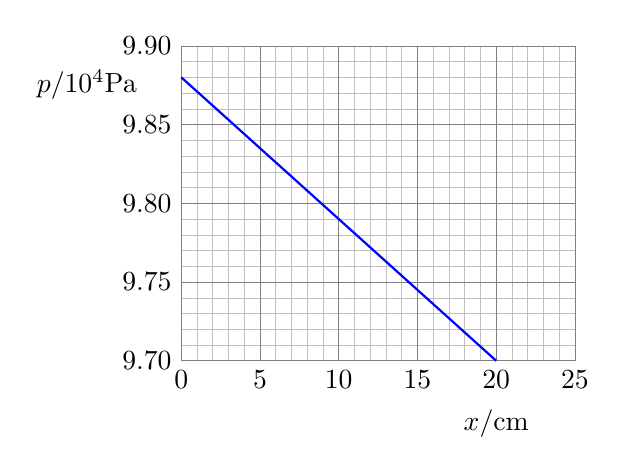
\begin{tikzpicture}
	\draw[help lines, gray!50, very thin, step=0.2] (0,0) grid (5,4);
	\draw[help lines, step=1] (0,0) grid (5,4);
	\foreach \y/\ylabel in {0/9.70,1/9.75,2/9.80,3/9.85, 4/9.90} \node[left] at (0,\y) {$\ylabel$};
	\foreach \x in {0,5,10,15,20,25} \node[below] at (\x/5,0) {$\x$};
	\node at (-1.2,3.5) {$p$/$10^4$Pa};
	\node at (4,-0.8) {$x$/cm};
	\draw[thick,blue] (0,3.6) -- (4,0);
	\end{tikzpicture}
	\vspace*{-25pt}
\end{marginfigure}

\example{The pressure $p$ of a liquid in a container varies with the height $x$ above the base of the container as shown. The total depth of the liquid is 20 cm. (a) What is the atmospheric pressure? (b) What is the density of the liquid?}

\sol surface of liquid at height $x= 20\text{ cm}$, so 

{
	\centering
	
	$P_\text{atm} = 9.70 \times10^4 \text{ Pa}$
	
}

density of liquid: $\rho = \frac{\Delta p}{g \Delta h} = \frac{(9.88-9.70)\times10^4}{9.81 \times 0.20} \RA \rho \approx 917 \text{ kg m}^{-3}$ \eoe



\subsection{pressure meters}

there are many types of instruments for pressure measurement

we would only focus on two: simple manometers and barometers
\footnote{Some examples of many other types of pressure gauges include
	
\begin{compactitem}
	
	\item[--] mechanical gauges based on metallic pressure-sensing elements
	
	\item[--] electronic gauges based on piezo-resistive effect
	
	\item[--] hot-filament ionization gauges based on ion currents from a gas

\end{compactitem}

Those who are interested are welcome to research into their functions and principles.
}

they both use the fact that $\Delta p = \rho g \Delta h$ within a liquid


\subsection{manometers}

\begin{marginfigure}
	\vspace*{-32pt}
	\centering
	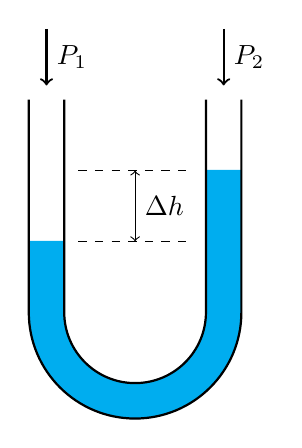
\begin{tikzpicture}[scale=0.9]
	\draw[cyan,fill] (1.5,2) -- (1.5,0) arc(0:-180:1.5) -- (-1.5,1) -- (-1,1) -- (-1,0) arc(-180:0:1) -- (1,2) -- cycle;
	\draw[thick] (1.5,3) -- (1.5,0) arc(0:-180:1.5) -- (-1.5,3)  (-1,3) -- (-1,0) arc(-180:0:1) -- (1,3);
	\draw[<->] (0,1) -- (0,2) node[right, midway] {$\Delta h$};
	\draw[dashed] (-0.8,1) --++ (1.6,0);
	\draw[dashed] (-0.8,2) --++ (1.6,0);
	\draw[thick,->] (-1.25,4) --++ (0,-0.8) node[midway,right]{$P_1$}; 
	\draw[thick,->] (1.25,4) --++ (0,-0.8) node[midway,right]{$P_2$}; 
	\end{tikzpicture}
	\vspace*{-16pt}
\end{marginfigure}

a \keypoint{manometer} consists of a U-shaped tube filled with some liquid

any pressure difference between the two ends of the tube could cause a height difference between liquid levels

for the situation shown, at equilibrium, one has: $P_1 - P_2 = \rho g \Delta h$

if $P_2$ is a reference pressure, then $P_1$ can be calculated

\cmt though any fluid can be used in a manometer, \emph{mercury} is preferred because of its high density ($\rho_\text{Hg} = 1.36 \times 10^4 \text{ kg m}^{-3}$)

\example{A manometer is used to measure the pressure of a gas supply. Side $A$ of the tube is connected to the gas pipe, and the other side $B$ of the tube is open to the atmosphere. If the mercury on side $A$ is higher than on side $B$ by 14 cm, what is the pressure of the gas? (density of mercury: $1.36 \times 10^4 \text{ kg m}^{-3}$; atmospheric pressure: $1.01 \times 10^5 \text{ Pa}$)}

\solc\begin{equation*}
	P_\text{atm} - P_\text{gas} = \rho g h \RA P_\text{gas} = 1.01 \times 10^5 - 1.36 \times 10^4 \times 9.81 \times 0.14 \RA P_\text{gas} \approx 8.23 \times 10^4 \text{ Pa} 
\end{equation*}


\subsection{barometers}

\begin{marginfigure}
	\vspace*{-5pt}
	\centering
	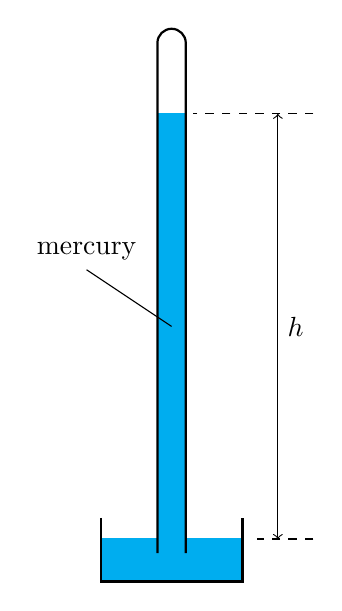
\begin{tikzpicture}[scale=0.9]
	\draw[cyan,fill] (-0.2,6) -- (0.2,6) -- (0.2,0) -- (1,0) -- (1,-0.6) -- (-1,-0.6) -- (-1,0) -- (-0.2,0) -- cycle;
	\draw[thick] (-1,0.3) -- (-1,-0.6) -- (1,-0.6) -- (1,0.3);
	\draw[thick] (-0.2,-0.2) -- (-0.2,7) arc(180:0:0.2) -- (0.2,-0.2);
	\draw (0,3) --++ (-1.2,0.8) node[above]{mercury};
	\draw[<->] (1.5,0) --++ (0,6) node[midway,right]{$h$};
	\draw[dashed] (2,6) -- (0.3,6);
	\draw[dashed] (2,0) -- (1.2,0);
	\end{tikzpicture}
	\vspace*{-16pt}
\end{marginfigure}


take a long glass tube and fill it with mercury

let it stand upside down in a basin

there is atmospheric pressure pushing down on surface of mercury, so a height of mercury is supported up the tube

we can then compute atmospheric pressure by: $P_\text{atm} = \rho g h$

this instrument makes a \keypoint{mercury barometer}

\example{If a mercury barometer supports a height of 760 mm of mercury above the fluid level in the container, what is the atmospheric pressure? If water is used as the barometric liquid, what is the minimum length of the tube required for the same atmospheric pressure? (density of mercury: $1.36 \times 10^4 \text{ kg m}^{-3}$; density of water: $1.00 \times 10^3 \text{ kg m}^{-3}$;)}

\sol atmospheric pressure: $P_\text{atm} = \rho g h = 1.36 \times 10^4 \times 9.81 \times 0.760 \approx 1.01\times10^5 \text{ Pa}$

if mercury is replaced by water: $h' = \frac{P_\text{atm}}{\rho' g} = \frac{1.01\times 10^5}{1000 \times 9.81} \approx 10.3 \text{ m}$ \eoe


\subsection{upthrust}

\begin{marginfigure}
	\vspace*{-8pt}
	\centering
	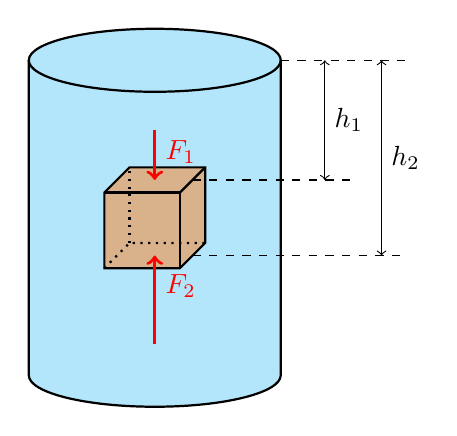
\begin{tikzpicture}[scale=0.8]
	\draw[thick,fill=cyan!30] (-2,2.5) arc(180:0:2 and 0.5) -- (2,-2.5) arc(0:-180:2 and 0.5) -- cycle;
	\draw[thick] (2,2.5) arc(0:-180:2 and 0.5);
	\draw[thick,fill=brown!60] (-0.8,-0.8) --++ (0,1.2) --++ (0.4,0.4) --++ (1.2,0) --++ (0,-1.2) --++ (-0.4,-0.4) -- cycle;
	\draw[thick] (-0.8,-0.8) ++ (0,1.2) --++ (1.2,0) --++ (0,-1.2);
	\draw[thick] (-0.8,-0.8) ++ (1.2,1.2) --++ (0.4,0.4);
	\draw[thick,dotted] (-0.8,-0.8)--++ (0.4,0.4) --++ (1.2,0);
	\draw[thick,dotted] (-0.8,-0.8) ++ (0.4,0.4) --++ (0,1.2);
	\draw[dashed] (2,2.5) -- (4,2.5);
	\draw[dashed] (0.6,0.6) -- (3.2,0.6);
	\draw[dashed] (0.6,-0.6) -- (4,-0.6);
	\draw[<->] (2.7,2.5) -- (2.7,0.6) node[right,midway]{$h_1$};
	\draw[<->] (3.6,2.5) -- (3.6,-0.6) node[right,midway]{$h_2$};
	\draw[very thick, red, ->] (0,1.4) -- (0,0.6) node[pos=.45, right]{$F_1$};
	\draw[very thick, red, ->] (0,-2) -- (0,-0.6) node[pos=0.65, right]{$F_2$};
	\end{tikzpicture}
%	\vspace*{-16pt}
\end{marginfigure}

now consider a rectangular block immersed in a fluid

top and bottom surface are at different depths, so they experience different pressures

this gives rise to an overall upward force on the cylinder

this force is called the \keypoint{upthrust}: \index{upthrust}
$$ F_U = F_2 - F_1 = \rho g (h_2 - h_1) \times A \RA \boxed{F_U = \rho g V} $$

therefore upthrust exerted on an immersed object equals the weight of the fluid displaced

this is known as the \keypoint{Archimedes' principle} \index{Archimedes' principle}

\cmt origin of upthrust: pressure difference between top and bottom surfaces

\cmt for an object of density $\rho_\text{o}$ immersed in a liquid of density $\rho_\text{l}$

take force in downward direction to be positive, then resultant force acting is:

{
	\centering
	
	$ \fnet = W - F_U = \rho_\text{o} g V - \rho_\text{l} g V = (\rho_\text{o} - \rho_\text{l}) gV$
	
}

\titem if $\rho_\text{o} > \rho_\text{l}$, then $\fnet>0$, resultant force acts downwards, object will sink

\titem if $\rho_\text{o} < \rho_\text{l}$, then $\fnet<0$, resultant force acts upwards, object will rise

\titem if $\rho_\text{o} = \rho_\text{l}$, then $\fnet=0$, object is in equilibrium, it can float at that level

\example{A block of mass 80 g and volume 50 cm$^3$ is suspended from a string into water. When the block is fully immersed and kept at rest, what is the tension in the string?}

\solc\begin{equation*}
	T + F_U = W \RA T = mg - \rho g V = 0.080 \times 9.81 - 1000 \times 9.81 \times 50 \times 10^{-6} \RA T \approx 0.29 \text{ N} 
\end{equation*}

\subsection{end-of-chapter questions}

Data for the questions below where applicable:

\titem density of water: $1.00 \times 10^3 \text{kg m}^{–3}$

\titem density of mercury: $13.6 \times 10^3 \text{kg m}^{–3}$

\titem atmospheric pressure: $1.0\times 10^5 \text{ Pa}$

\subsection*{pressure in a fluid}

\question{
	(a) A dam holds a depth of 50 m of water. What is the water pressure at the base of the dam? (b) Suggest why the walls of a dam must be made thicker near the bottom?
}

\question{
	The deepest trench on Earth is The Mariana Trench located in the Pacific Ocean. The maximum known depth is about 11 km. (a) Assume the sea water has a uniform density of about $1030 \text{ kg m}^{-3}$, estimate the pressure at the base of the trench. (b) The density of sea water actually increases slightly with pressure, suggest how this affects the result you have found.
}

\question{
	Instead of a large viewing window, the window of a submarine is usually of only a few centimetres in diameter. Why is the window made so small?
}

\question{
	If you punch several holes in the bottom of a container filled with water, water will spurt out due to the pressure. Now drop the container, suggest what will happen as it falls freely and defend your explanation.
}

\question{
	Air trapped inside a cylinder is attached to a U-shaped manometer containing mercury. The other side of the manometer is open to  atmosphere. The mercury column on the side open to atmosphere is found to be 45 mm higher, what is the pressure of the trapped air?
}

\begin{marginfigure}
	\vspace*{0pt}
	\centering
	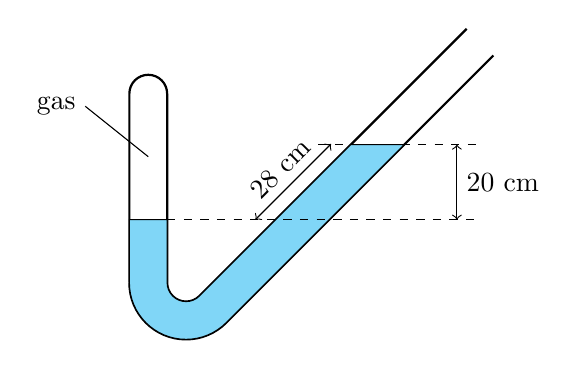
\begin{tikzpicture}[scale=0.8]
	\draw[thick] (0,0) -- (0,3) arc(180:0:0.3) -- (0.6,0) arc(180:315:0.3) --++ (45:6);
	\draw[thick] (0,0) arc(180:315:0.9) --++ (45:6);
	\draw[fill=cyan!50] (0,1) -- (0,0) arc(180:315:0.9) --++ (45:4) --++ (-0.8485,0) --++ (225:3.4) arc(315:180:0.3) -- (0.6,1) -- cycle;
	\draw (0.3,2) --++ (-1,0.8) node[left]{gas};
	\draw[dashed] (0.6,1) -- (5.6,1);
	\draw[dashed] (3,2.192) -- (5.6,2.192);
	\draw[<->] (5.2,1) -- (5.2,2.192) node[midway, right]{20 cm};
	\draw[<->] (2,1) --++ (45:1.7) node[midway, above, rotate=45]{28 cm};
	\end{tikzpicture}
	\vspace*{-12pt}
\end{marginfigure}

\question{The figure shows a pipe closed at one end and open at the other end. Some gas is trapped by a column of mercury as shown. Find the pressure of the gas.}

\question{A water manometer is used to measure the pressure created in a flexible container. Initially, the water columns on each side of the manometer is at the same level. When a girl stands on a 30 cm by 30 cm platform placed on top of the container, a height difference of 50 cm is observed in the manometer. (a) Find the pressure created by the girl. (b) Find the mass of the girl.}

\subsection*{upthrust}

\question{A lead block and an aluminium block of identical size are immersed in water. Upon which block is the upthrust greater?}

\question{
	If somehow the gravitational field on the earth is increased, does a fish sink, float to the surface, or otherwise?
}

\question{
	A diver holds a cube of side 0.30 m and density $800 \text{kg m}^{–3}$ near the seabed. (a) What is the upthrust on the cube? (b) What is its initial acceleration when the cube is released from rest?
}

\question{
	A solid sphere of radius 18 cm and density $2.4 \text{g cm}^{–3}$ is fully submerged in water. A string pulls on the sphere so that the sphere does not sink. (a) Find the tension in the string. (b) If the string is cut, what is the instantaneous acceleration. (c) Describe and explain the acceleration of the sphere as it sinks.
}